% Unofficial University of Cambridge Poster Template
% https://github.com/andiac/gemini-cam
% a fork of https://github.com/anishathalye/gemini
% also refer to https://github.com/k4rtik/uchicago-poster

\documentclass[final]{beamer}

% ====================
% Packages
% ====================

\usepackage[T1]{fontenc}
\usepackage{lmodern}
\usepackage[orientation=portrait,size=a0,scale=1.0]{beamerposter}
\usetheme{gemini}
\usecolortheme{nott}
\usepackage{graphicx}
\usepackage{booktabs}
\usepackage{tikz}
\usepackage{pgfplots}
\pgfplotsset{compat=1.14}
\usepackage{anyfontsize}


% for tables
\usepackage{multirow}
\usepackage{multicol}
\usepackage{transparent}

% for urls
\usepackage{hyperref}

% for subfigures
\usepackage{caption}
\usepackage{subcaption}

% for bibliography
\renewcommand{\refname}{Literature}
\usepackage[backend=biber]{biblatex}
\addbibresource{poster.bib} % Replace with your .bib file


% ====================
% Lengths
% ====================

% If you have N columns, choose \sepwidth and \colwidth such that
% (N+1)*\sepwidth + N*\colwidth = \paperwidth
\newlength{\sepwidth}
\newlength{\colwidth}
\setlength{\sepwidth}{0.025\paperwidth}
\setlength{\colwidth}{0.45\paperwidth}

\newcommand{\separatorcolumn}{\begin{column}{\sepwidth}\end{column}}

% ====================
% Title
% ====================

% Title page
\title{Network Diffusion --- Framework to Simulate Spreading Processes in Complex Networks}
\author{
    \textbf{Micha{\l} Czuba} \inst{1},
    Mateusz Nurek \inst{1},
    Damian Serwata \inst{1},
    Yu-Xuan Qi \inst{2},
    Mingshan Jia \inst{2},
    Katarzyna Musial \inst{2},
    Rados{\l}aw Michalski \inst{1},
    Piotr Br{\'o}dka \inst{1}
}
\institute[]{
  \inst{1} Wroc{\l}aw University of Science and Technology\\
  \inst{2} University of Technology Sydney
}

% ====================
% Footer (optional)
% ====================

\footercontent{
  \href{https://networks.pwr.edu.pl/}{https://networks.pwr.edu.pl} \hfill
  NetSci, Canada, July 2023 \hfill
  \href{mailto:michal.czuba@pwr.edu.pl}{michal.czuba@pwr.edu.pl}}

% ====================
% Logo (optional)
% ====================

\logoright{
\includegraphics[height=3.8cm]{logos/nsl-white.pdf}}
\logoleft{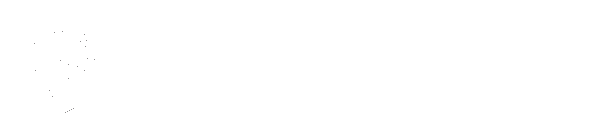
\includegraphics[height=3.8cm]{logos/wust_logo.pdf}}

% ====================
% Body
% ====================

\begin{document}

\begin{frame}[t]
\begin{columns}[t]

\separatorcolumn
\begin{column}{\colwidth}

\begin{block}{Introduction}
    The problem of selecting an optimal seed set to maximise influence in networks has been a subject of intense research in recent years. However, there is still a missing part to be tackled: \textbf{multilayer networks}. Methods robust for one-layer-graphs are not easily applicable to their multilayer counterparts. That narrows their usability in real-case scenarios such as marketing campaigns, misinformation tracking, or epidemiology, where multilayer networks usually express actual conditions better. \textbf{In this work, we show the efficiency of various metrics used to determine the initial seed set for the Multilayer Linear Threshold Model} (MLTM).
\end{block}

\begin{alertblock}{Extending the LTM to multilayer networks}
    Linear Threshold Model in its initial form~\cite{kempe2003maximizing} cannot be directly applied to multilayer networks --- \textbf{actors are the subject of the process, while the nodes are their auxiliary representation}...
    Therefore, we need to define:
    \begin{itemize}
        \item what does it mean that an actor is (or is not) active,
        \item how does it relate to diffusion dynamics taking place within 
        layers, where it is represented.
    \end{itemize}
    In our research, we used the approach proposed by~\cite{zhong2022mltm} with amendments so that a homogeneity among actors has been imposed in the sense of an activation threshold ($\mu$) and a protocol (v.i.).

    \heading{Protocol function in MLTM}\label{def:proto}
        According to~\cite{zhong2022mltm}, state of the actor $n$ of a multilayer network $M = (N, L, V, E)$ in the time step $t$ is determined
        by a following function: 
        \begin{equation*}
            x_{n}(t) =
            \begin{cases}
              1,  & \text{if \space} y_{n}(t) \geq \delta \text{\space or 
                \space} x_{n}(t-1) = 1 \\
              0,  & \text{otherwise}
            \end{cases} 
        \end{equation*}
        Where:
        \begin{description}
            \item[$\delta$] - a parameter of the model, $\delta \in [\frac{1}{|L|}, 1]$,
            \item[$y_{n}(t)$] - a mean input of actor $n$ (represented in $K$ layers) in time $t$, $y_{n}(t) = |K|^{-1} \sum_{k \in K} y_{v}^{k}(t)$.
            \item[$y_{v}^{k}(t)$] - an impulse of node $v$ from layer $k$ in time $t$, $y_{v}^{k}(t) \in \{0, 1\}$
        \end{description}

    \heading{Toy example}
    \textbf{We decided to examine two extreme cases: $\mathbf{\delta = 1}$ ($\mathbf{AND}$) and $\mathbf{delta = \frac{1}{L}}$ ($\mathbf{OR}$)}. In the former one, an actor gets activated if it receives sufficient influence on all layers where it is represented, and conversely the latter, where sufficient input in at least one layer is enough for activation.
    \begin{figure}
        \centering
        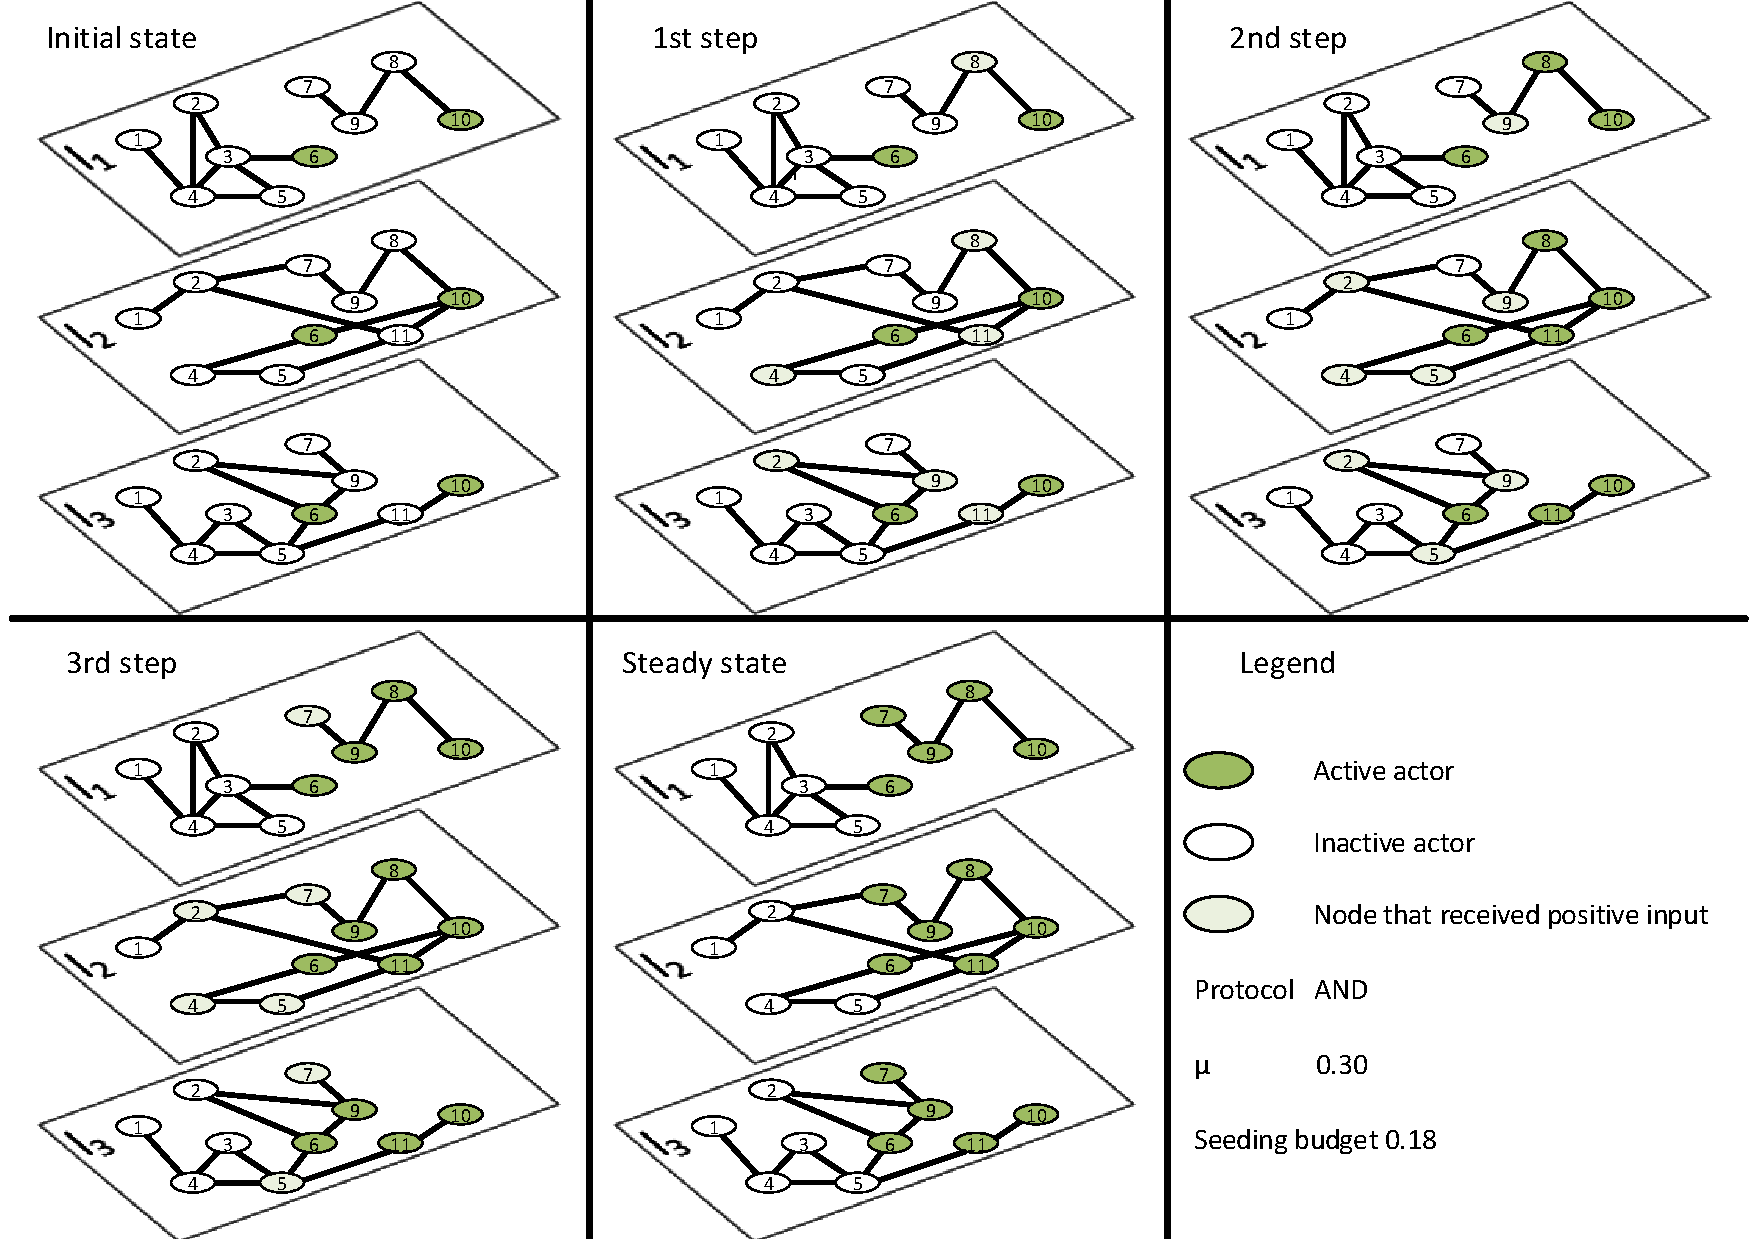
\includegraphics[width=1\linewidth]{figures/ltm_example.pdf}
        \caption{Example of spreading of MLTM in toy network with protocol $AND$.}
        \label{fig:ltm_example_and}
    \end{figure}
\end{alertblock}

\begin{block}{A problem we tackled}
    \heading{Budget constrained influence maximisation}
    Let $\mathcal{S}$ be a family of sets of cardinality $s$ over actors of
    the multilayer network $M$ in the sense that $\mathcal{S} \subseteq
    powerset(N)$. Let $\sigma: \mathcal{S} \rightarrow \mathbb{R^{+}}$ b
    an arbitrary function that maps a set of actors used as a seed set to
    a number denoting the expected size of activated actors in a binary discrete system. An influence maximisation problem for seeding budget of size $s$ is an issue of finding $ S_{0}: \arg\max(\sigma) = S_{0} \wedge |S_{0}| \leq s$.
    
    \heading{Measuring an efficiency of the diffusion}
    We used \textbf{Gain} metric to assess a performance of the spreading model that bases on a number of seeds, a number of actors that could be activated, and a number of active actors when diffusion faded down:
    \begin{equation*}
        G = 100 \cdot \frac{|S_{D} - S_{0}|}{|N - S_{0}|}
    \end{equation*}
\end{block}

\begin{block}{Seed selection methods}
    During the study, we evaluated the following methods to select seed set for MLTM:
    \begin{itemize}
        \item degree (\textit{deg-c)},
        \item neighbourhood size (\textit{nghb-1s}, \textit{nghb-2s}),
        \item PageRank (\textit{p-rnk}, \textit{p-rnk-m}),
        \item VoteRank (\textit{v-rnk}, \textit{v-rnk-m}),
        \item k-shell decomposition (\textit{k-sh}, \textit{k-sh-m}),
        \item random choice (\textit{random}),
        \item greedy (\textit{greedy}).
    \end{itemize}
    We used two ideas to adapt PageRank, VoteRank, and k-shell to multilayer networks: compute the metric for each layer and take its mean value for each actor (e.g. \textit{p-rnk}) or replace Degree Centrality with Neighbourhood Size in the algorithm (e.g. \textit{p-rnk-m}).
\end{block}

\end{column}

\separatorcolumn
\begin{column}{\colwidth}

\begin{block}{Used data and parameter space}
    \begin{table}
    \begin{subtable}[t]{0.45\textwidth}
        \caption{}
        \resizebox{\columnwidth}{!}{%
            \begin{tabular}{lllllp{14cm}}
                \hline Name & Layers & Actors & Nodes & Edges & Note \\ \hline
                aucs & 5 & 61 & 224 & 620 & AUCS CS-AARHUS \\
                ckmp & 3 & 241 & 674 & 1370 & Coleman, Katz, Menzel Innovation Among Physicians \\
                eutr-A & 37 & 417 & 2034 & 3588 & The European Air Transport Network \\
                lazega & 3 & 71 & 212 & 1659 & Lazega Law Firm \\ \hline
                er-2 & 2 & 1000 & 2000 & 5459 & \multirow{3}{*}{\parbox{14cm}{Erdős–Rényi networks generated with multinet library}} \\
                er-3 & 3 & 1000 & 3000 & 7136 & \\
                er-5 & 5 & 1000 & 5000 & 15109 & \\ \hline
                sf-2 & 2 & 1000 & 2000 & 4223 & \multirow{3}{*}{\parbox{14cm}{Scale-free networks generated with multinet library}} \\
                sf-3 & 3 & 1000 & 3000 & 5010 & \\
                sf-5 & 5 & 1000 & 5000 & 10181 & \\ \hline
            \end{tabular}%
        }
        \label{tab:networks_eda}
    \end{subtable}
    \hspace{\fill}
    \begin{subtable}[t]{0.45\textwidth}
        \caption{}
        \resizebox{\columnwidth}{!}{%
        \begin{tabular}{lp{10cm}p{10cm}}
            Protocol & $OR$ & $AND$ \\ \hline
            $s$ range & $[1, 2, ..., 10, 15, 20, 25, 30]$ & $[15, 20, 25, 30, 31, ..., 40]$ \\ \hline
            $\mu$ range & \multicolumn{2}{p{20cm}}{$[0.1, 0.2, 0.3, 0.4, 0.5, 0.6, 0.7, 0.8, 0.9]$} \\ \hline
            networks & \multicolumn{2}{p{20cm}}{real (aucs, ckmp, lazega, eutr-A), Erdős–Rényi (er-2, er-3, er-5), Scale-free (sf-2, sf-3, sf-5)} \\ \hline
            s.~s.~method & \multicolumn{2}{p{20cm}}{deg-c, greedy, k-sh, k-sh-m, nghb-1s, nghb-2s, p-rnk, p-rnk-m, random, v-rnk, v-rnk-m} \\
        \end{tabular}%
        }
        \label{tab:parameter_space}
    \end{subtable}
    \caption{Networks used in experiments with their basic parameters shortlisted (tab.~\ref{tab:networks_eda}), values of each evaluated parameter - in total 27,720 executed experiments (tab.~\ref{tab:parameter_space}).}
    \end{table}
\end{block}

\begin{block}{Initial results}
    \begin{figure}
        \centering
        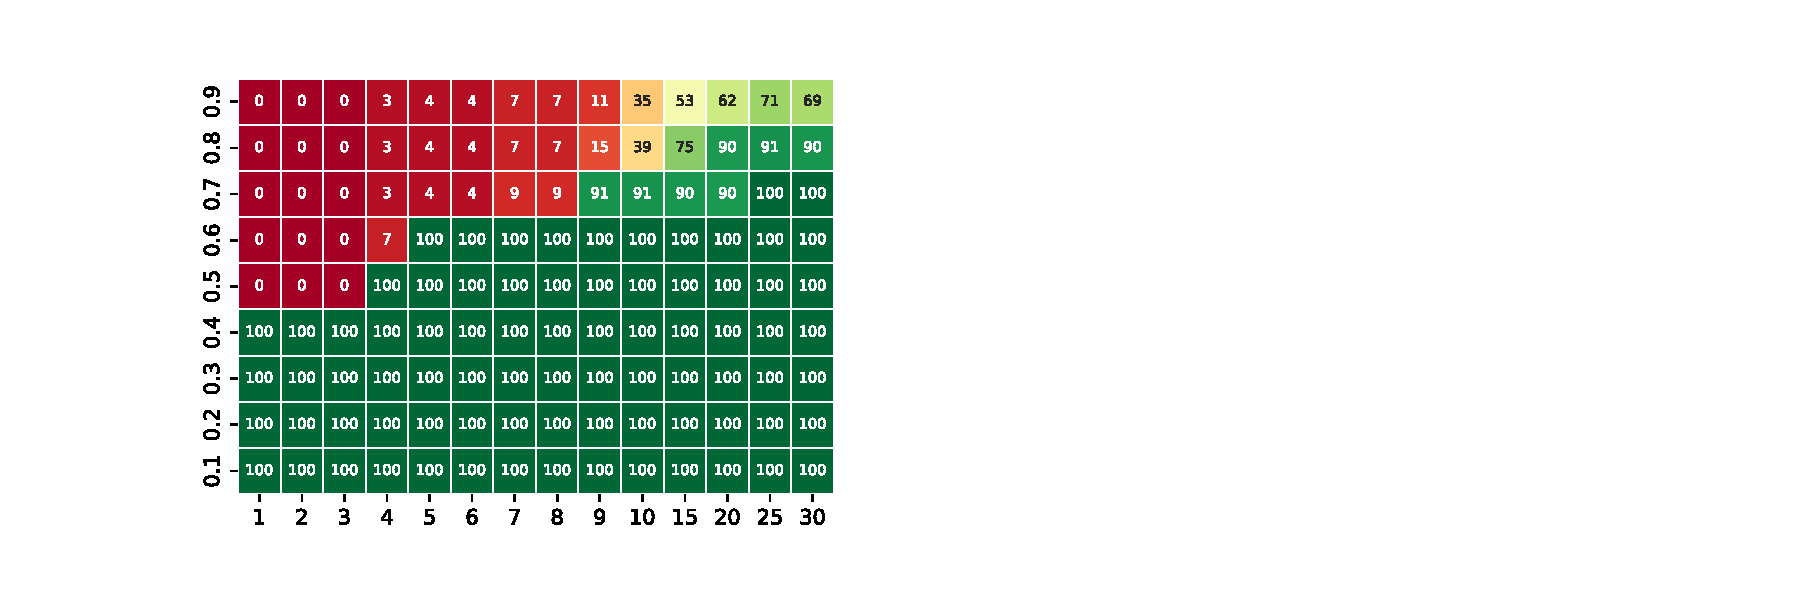
\includegraphics[width=.24\textwidth]{figures/robustness_maps/raw_gain_v-rnk-m.pdf}
        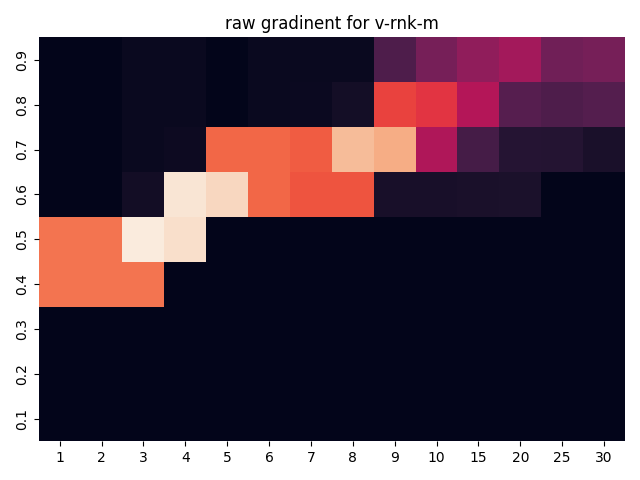
\includegraphics[width=.24\textwidth]{figures/robustness_maps/raw_grad_v-rnk-m.png}
        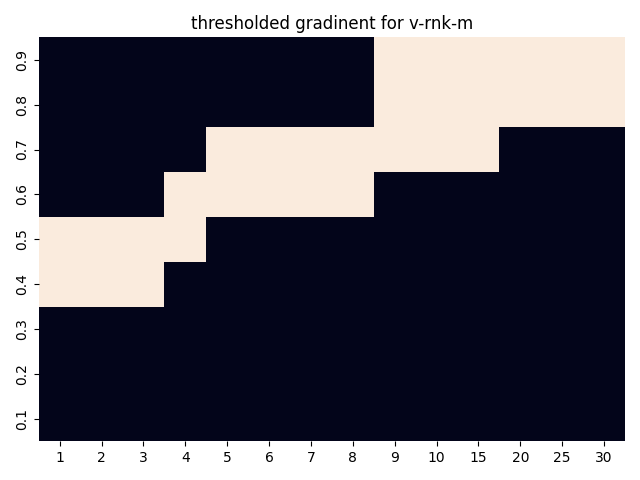
\includegraphics[width=.24\textwidth]{figures/robustness_maps/thre_grad_v-rnk-m.png}
        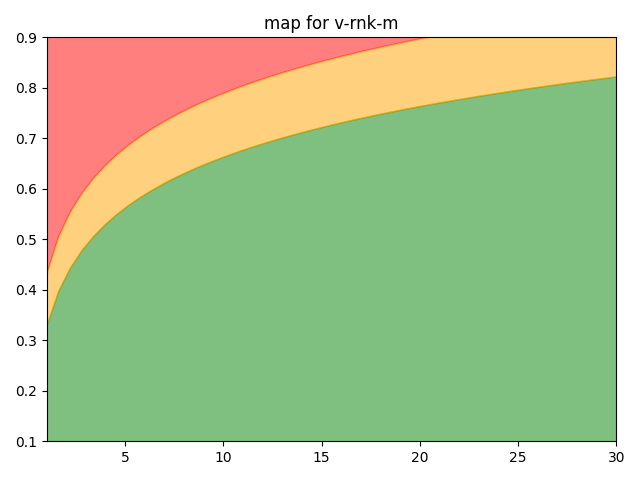
\includegraphics[width=.24\textwidth]{figures/robustness_maps/rob_map_v-rnk-m.png}
        \caption{Example of three zones on $G$ heatmap for the \textit{v-rnk-m} method on \textit{aucs} network with protocol \textit{OR}. 
        (1) a heatmap of the raw gain, (2) computed gradient magnitude,
        (3) thresholded gradient that divides the area into three sections, and (4) the final division of the $\mu~\times~s~\times~G$ space.}
        \label{fig:rm_example}
    \end{figure}

    We observed:
    \begin{itemize}
        \item existence of three areas on the heatmaps (“robust”, “transitional”, and “unrobust”),
        \item that length of the diffusion is highest in the “transitional” zone,
        \item for Erdős-Rényi networks the transitional zone is the narrowest,
        \item for Scale-Free networks transitional zone is typically present,
        \item for real networks the most significant differences between the $\mu~\times~s~\times~G$ heatmaps.
    \end{itemize}

\end{block}

\begin{block}{Coarse assessment of seed selection methods}
    \begin{figure}
        \centering
        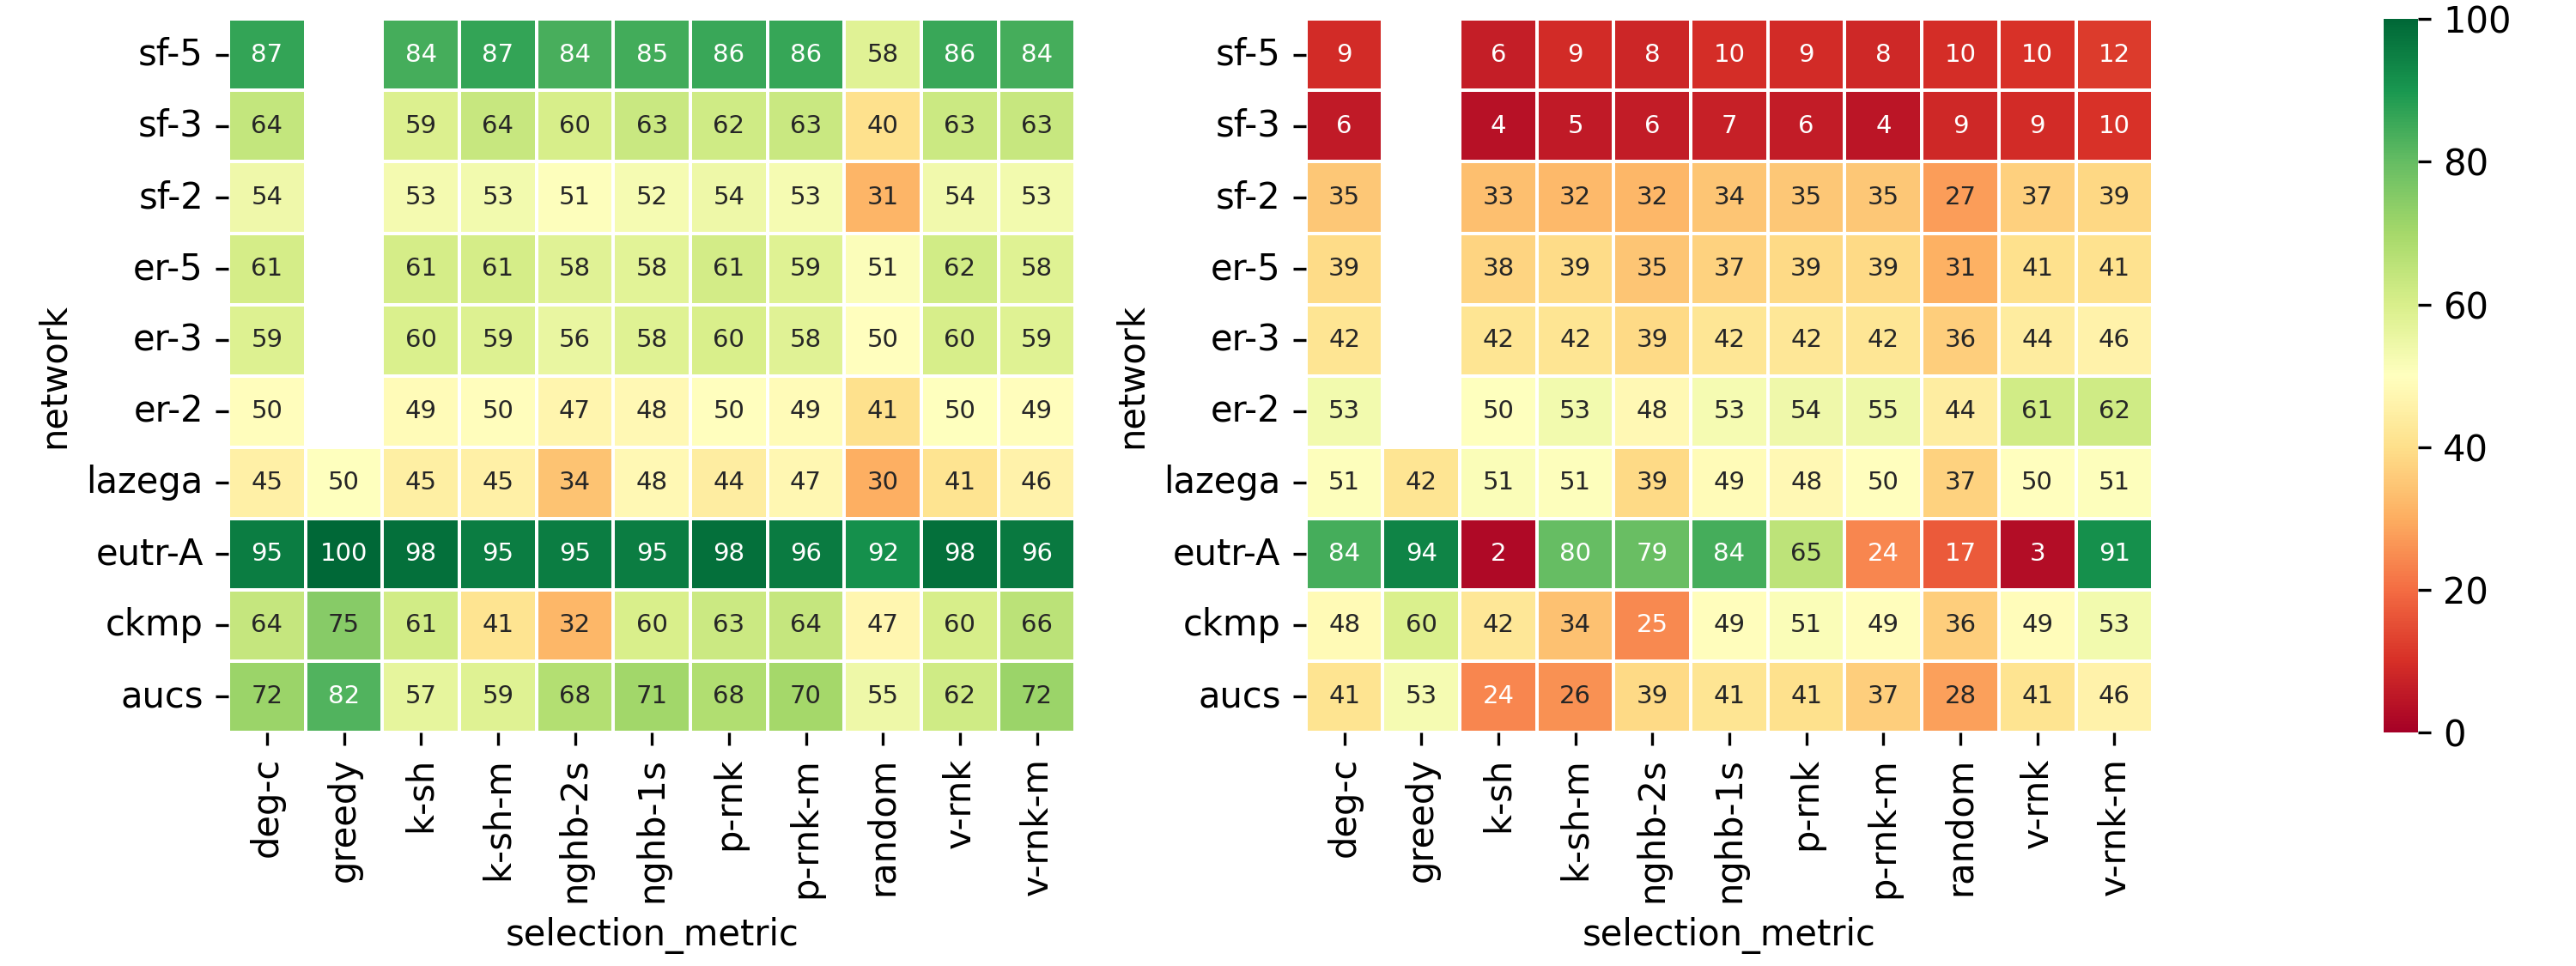
\includegraphics[width=1\linewidth]{figures/means_multilayer.png}
        \caption{Heatmaps of mean $G$ achieved by evaluated seed 
        selection methods on multilayer networks. \textbf{Left:} protocol 
        $OR$. \textbf{Right:} protocol $AND$.}
        \label{fig:mean_gain_mln}
    \end{figure}
    We observed:
    \begin{itemize}
        \item network type impacts the $G$, surpassing the influence of seed selection methods,
        \item $random$ and $greedy$ stand out of the another methods.
        \item network topology strongly affects efficiency of MLTM diffusion (more layers lead to better $G$ for $OR$, whereas worse $G$ for $AND$),
        \item most of the evaluated methods behave similarly regarding the network for which they are applied.
    \end{itemize}
\end{block}

\begin{block}{Rankings of seed selection methods}
    \begin{table}
    \begin{subtable}{0.45\textwidth}
        \caption{}
        \resizebox{\columnwidth}{!}{%
        \begin{tabular}{ccccc}
            Seed Selection Method & \multicolumn{4}{c}{Networks} \\
            & Real & Erdős–Rényi & Scale-free & All \\ \hline
            deg-c & 3.12 & 4.57 & 5.55 & 4.28 \\
            greedy & \textbf{1.33} & \multicolumn{3}{c}{not computed}\\
            k-sh    & 5.46 & 4.82 & 7.95 & 6.02 \\
            k-sh-m  & 4.58 & 4.63 & 6.31 & 5.11 \\
            nghb-2s & 4.14 & 5.44 & 6.53 & 5.25 \\
            nghb-1s & 2.91 & 4.22 & 5.18 & 3.99 \\
            p-rnk   & 3.05 & 3.60 & 5.02 & 3.81 \\
            p-rnk-m & 3.87 & 3.94 & 6.51 & 4.68 \\
            random  & 5.23 & 5.42 & 6.74 & 5.74 \\
            v-rnk   & 3.93 & 3.08 & 4.36 & 3.80 \\
            v-rnk-m & 2.11 & \textbf{3.04} & \textbf{2.85} & \textbf{2.61} \\ \hline
        \end{tabular}%
        }
        \label{tab:ranking_or_mln}
    \end{subtable}
    \hspace{\fill}
    \begin{subtable}{0.45\textwidth}
        \caption{}
        \resizebox{\columnwidth}{!}{%
        \begin{tabular}{ccccc}
        Seed Selection Method & \multicolumn{4}{c}{Networks} \\
        & Real & Erdős–Rényi & Scale-free & All \\ \hline
        deg-c &  2.57 & 3.20 & \textbf{2.90} & 2.86 \\
        greedy & \textbf{1.03} & \multicolumn{3}{c}{not computed}\\
        k-sh    & 2.67 & 3.20 & 3.69 & 3.13 \\
        k-sh-m  & 3.03 & 3.23 & 3.18 & 3.13 \\
        nghb-2s & 3.31 & 3.93 & 4.26 & 3.78 \\
        nghb-1s & 2.72 & 3.43 & 3.67 & 3.22 \\
        p-rnk   & 2.31 & 2.83 & 3.04 & 2.69 \\
        p-rnk-m & 2.57 & 2.98 & 3.54 & 2.99 \\
        random  & 3.44 & 4.55 & 4.54 & 4.10  \\
        v-rnk   & 2.62 & \textbf{2.34} & 2.92 & \textbf{2.62} \\
        v-rnk-m & 2.35 & 3.53 & 3.49 & 3.05 \\ \hline
        \end{tabular}%
        }
        \label{tab:ranking_and_mln}
    \end{subtable}
    \caption{Rankings of seed selection methods with respect to the achieved $G$ for protocols $OR$ (tab.~\ref{tab:ranking_or_mln}) and $AND$ tab.~\ref{tab:ranking_and_mln}) grouped by graph type (the higher number the better).}
    \label{tab:ranking_mln}
    \end{table}
\end{block}
    
\begin{exampleblock}{Conclusions}
    \begin{itemize}
        \item we confirmed that efficiency of centrality based heuristics is located between \textit{random} and \textit{greedy},
        \item we have proposed an extension of VoteRank, PageRank and k-shell to multilayer networks,
        \item for both protocols VoteRank is the most efficient method,
        \item in real case scenarios, it could be better to make the $\mu$ smaller (i.e. invest in a mass marketing) than to put efforts in selecting the optimal $S_{0}$ (i.e. conduct the campaign with influencers).
    \end{itemize}
\end{exampleblock}

\begin{block}{References}
    % \nocite{*}
    % \footnotesize{\bibliographystyle{ieeetr}\bibliography{poster}}
    \printbibliography
\end{block}

\end{column}
\separatorcolumn

\end{columns}
\end{frame}

\end{document}
